\documentclass{standalone}
\usepackage{tikz}
\usetikzlibrary{patterns}
\usetikzlibrary{positioning}
\usetikzlibrary{patterns, positioning}
\usetikzlibrary{shapes.misc}
\usepackage[outline]{contour}
\contourlength{1.5pt} 
\usetikzlibrary{calc}
        \usepackage{relsize}
        \tikzset{fontscale/.style = {font=\relsize{#1}}}

\begin{document}
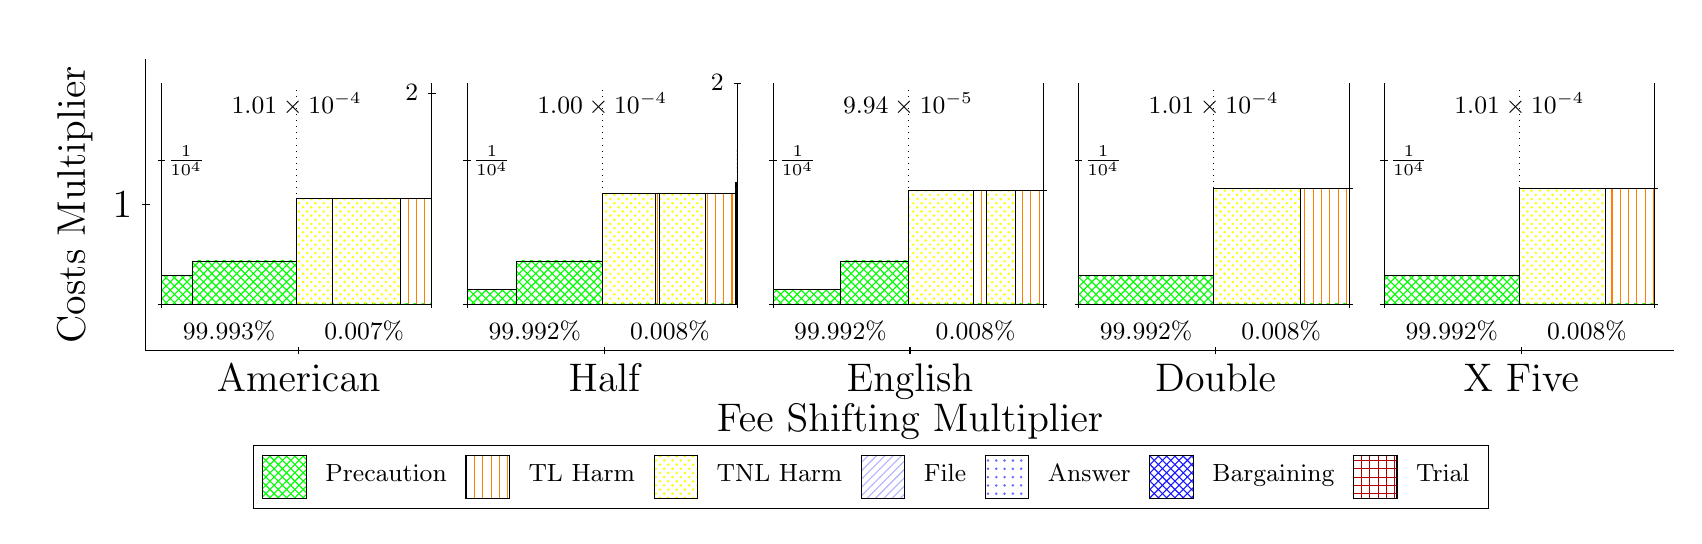
\begin{tikzpicture}
\clip(-0.5,-1.1) rectangle +(20.91,6.2);
\draw[black] (1,1) -- (1,4.7);
\node[rotate=90, fontscale=2, anchor=center] at (0.1, 2.85) {Costs Multiplier};
\draw[black] (0.95,2.85) -- (1.05,2.85);
\node[fontscale=2, anchor=east] at (0.95, 2.85) {1};

\draw[black] (1,1) -- (20.41,1);
\node[fontscale=2, anchor=center] at (10.705, 0.1) {Fee Shifting Multiplier};
\draw[black] (2.941,0.95) -- (2.941,1.05);
\node[fontscale=2, anchor=north] at (2.941, 0.95) {American};
\draw[black] (6.823,0.95) -- (6.823,1.05);
\node[fontscale=2, anchor=north] at (6.823, 0.95) {Half};
\draw[black] (10.705,0.95) -- (10.705,1.05);
\node[fontscale=2, anchor=north] at (10.705, 0.95) {English};
\draw[black] (14.587,0.95) -- (14.587,1.05);
\node[fontscale=2, anchor=north] at (14.587, 0.95) {Double};
\draw[black] (18.469,0.95) -- (18.469,1.05);
\node[fontscale=2, anchor=north] at (18.469, 0.95) {X Five};


\draw[pattern=crosshatch, pattern color=green,draw=black,very thin] (1.2,1.592) rectangle (1.5947,1.9555);
\draw[pattern=crosshatch, pattern color=green,draw=black,very thin] (1.5947,1.592) rectangle (2.916,2.1373);
\draw[pattern=crosshatch, pattern color=green,draw=black,very thin] (2.916,1.592) rectangle (3.3705,1.592);
\draw[pattern=crosshatch dots, pattern color=yellow,draw=black,very thin] (2.916,1.592) rectangle (3.3705,2.9323);
\draw[pattern=crosshatch, pattern color=green,draw=black,very thin] (3.3705,1.592) rectangle (3.3737,1.592);
\draw[pattern=vertical lines, pattern color=orange,draw=black,very thin] (3.3705,1.592) rectangle (3.3737,2.9323);
\draw[pattern=crosshatch, pattern color=green,draw=black,very thin] (3.3737,1.592) rectangle (4.229,1.592);
\draw[pattern=crosshatch dots, pattern color=yellow,draw=black,very thin] (3.3737,1.592) rectangle (4.229,2.9323);
\draw[pattern=crosshatch, pattern color=green,draw=black,very thin] (4.229,1.592) rectangle (4.6301,1.592);
\draw[pattern=vertical lines, pattern color=orange,draw=black,very thin] (4.229,1.592) rectangle (4.6301,2.9323);
\draw[pattern=crosshatch, pattern color=green,draw=black,very thin] (4.6301,1.592) rectangle (4.6313,1.592);
\draw[pattern=crosshatch dots, pattern color=yellow,draw=black,very thin] (4.6301,1.592) rectangle (4.6313,2.9323);
\draw[pattern=north east lines, pattern color=blue!30,draw=black,very thin] (4.6301,2.9323) rectangle (4.6313,3.0663);
\draw[pattern=dots,  pattern color=blue!60,draw=black,very thin] (4.6301,3.0663) rectangle (4.6313,3.2004);
\draw[pattern=crosshatch,      pattern color=blue!90,draw=black,very thin] (4.6301,3.2004) rectangle (4.6313,3.4684);
\draw[pattern=grid,            pattern color=red!70!black,draw=black,very thin] (4.6301,3.4684) rectangle (4.6313,3.7365);
\draw[pattern=crosshatch, pattern color=green,draw=black,very thin] (4.6313,1.592) rectangle (4.632,1.592);
\draw[pattern=vertical lines, pattern color=orange,draw=black,very thin] (4.6313,1.592) rectangle (4.632,2.9323);
\draw[pattern=north east lines, pattern color=blue!30,draw=black,very thin] (4.6313,2.9323) rectangle (4.632,3.0663);
\draw[pattern=dots,  pattern color=blue!60,draw=black,very thin] (4.6313,3.0663) rectangle (4.632,3.2004);
\draw[pattern=crosshatch,      pattern color=blue!90,draw=black,very thin] (4.6313,3.2004) rectangle (4.632,3.4684);
\draw[pattern=grid,            pattern color=red!70!black,draw=black,very thin] (4.6313,3.4684) rectangle (4.632,3.7365);
\node[font=\small,text=black,anchor=north] at (2.916, 4.4) {$1.01\times 10^{-4}$};
\draw[black,very thin] (1.2,1.592) -- (1.2,4.4);
\draw[black,very thin] (1.15,1.592) -- (1.25,1.592);
\node[font=\small,text=black, anchor=west] at (1.15, 1.592) {};
\draw[black,very thin] (1.15,3.4097) -- (1.25,3.4097);
\node[font=\small,text=black, anchor=west] at (1.15, 3.4097) {$\frac{1}{10^{4}}$};

\draw[black,dotted,very thin] (2.916,1.6762) -- (2.916,4.3158);
\draw[black,very thin] (4.632,1.592) -- (4.632,4.4);
\draw[black,very thin] (4.582,4.2726) -- (4.682,4.2726);
\node[font=\small,text=black, anchor=east] at (4.582, 4.2726) {\contour{white}{2}};

\draw[black,very thin] (1.2,1.592) -- (4.632,1.592);
\draw[black,very thin] (1.2,1.542) -- (1.2,1.642);
\node[font=\small,text=black, anchor=north] at (1.2, 1.542) {};
\draw[black,very thin] (4.632,1.542) -- (4.632,1.642);
\node[font=\small,text=black, anchor=north] at (4.632, 1.542) {};

\node[font=\small,text=black,anchor=south] at (2.058, 0.992) {99.993\%};
\node[font=\small,text=black,anchor=south] at (3.774, 0.992) {0.007\%};

\draw[pattern=crosshatch, pattern color=green,draw=black,very thin] (5.082,1.592) rectangle (5.7085,1.7738);
\draw[pattern=crosshatch, pattern color=green,draw=black,very thin] (5.7085,1.592) rectangle (6.798,2.1373);
\draw[pattern=crosshatch, pattern color=green,draw=black,very thin] (6.798,1.592) rectangle (6.7987,1.592);
\draw[pattern=north east lines, pattern color=blue!30,draw=black,very thin] (6.798,1.592) rectangle (6.7987,1.7324);
\draw[pattern=dots,  pattern color=blue!60,draw=black,very thin] (6.798,1.7324) rectangle (6.7987,1.8728);
\draw[pattern=crosshatch,      pattern color=blue!90,draw=black,very thin] (6.798,1.8728) rectangle (6.7987,2.1536);
\draw[pattern=crosshatch, pattern color=green,draw=black,very thin] (6.7987,1.592) rectangle (7.4764,1.592);
\draw[pattern=crosshatch dots, pattern color=yellow,draw=black,very thin] (6.7987,1.592) rectangle (7.4764,2.996);
\draw[pattern=crosshatch, pattern color=green,draw=black,very thin] (7.4764,1.592) rectangle (7.5221,1.592);
\draw[pattern=vertical lines, pattern color=orange,draw=black,very thin] (7.4764,1.592) rectangle (7.5221,2.996);
\draw[pattern=crosshatch, pattern color=green,draw=black,very thin] (7.5221,1.592) rectangle (8.111,1.592);
\draw[pattern=crosshatch dots, pattern color=yellow,draw=black,very thin] (7.5221,1.592) rectangle (8.111,2.996);
\draw[pattern=crosshatch, pattern color=green,draw=black,very thin] (8.111,1.592) rectangle (8.4905,1.592);
\draw[pattern=vertical lines, pattern color=orange,draw=black,very thin] (8.111,1.592) rectangle (8.4905,2.996);
\draw[pattern=crosshatch, pattern color=green,draw=black,very thin] (8.4905,1.592) rectangle (8.4944,1.592);
\draw[pattern=crosshatch dots, pattern color=yellow,draw=black,very thin] (8.4905,1.592) rectangle (8.4944,2.996);
\draw[pattern=north east lines, pattern color=blue!30,draw=black,very thin] (8.4905,2.996) rectangle (8.4944,3.1364);
\draw[pattern=crosshatch, pattern color=green,draw=black,very thin] (8.4944,1.592) rectangle (8.5058,1.592);
\draw[pattern=vertical lines, pattern color=orange,draw=black,very thin] (8.4944,1.592) rectangle (8.5058,2.996);
\draw[pattern=north east lines, pattern color=blue!30,draw=black,very thin] (8.4944,2.996) rectangle (8.5058,3.1364);
\draw[pattern=crosshatch, pattern color=green,draw=black,very thin] (8.5058,1.592) rectangle (8.5092,1.592);
\draw[pattern=crosshatch dots, pattern color=yellow,draw=black,very thin] (8.5058,1.592) rectangle (8.5092,2.996);
\draw[pattern=north east lines, pattern color=blue!30,draw=black,very thin] (8.5058,2.996) rectangle (8.5092,3.1364);
\draw[pattern=dots,  pattern color=blue!60,draw=black,very thin] (8.5058,3.1364) rectangle (8.5092,3.2768);
\draw[pattern=crosshatch,      pattern color=blue!90,draw=black,very thin] (8.5058,3.2768) rectangle (8.5092,3.5576);
\draw[pattern=crosshatch, pattern color=green,draw=black,very thin] (8.5092,1.592) rectangle (8.5119,1.592);
\draw[pattern=vertical lines, pattern color=orange,draw=black,very thin] (8.5092,1.592) rectangle (8.5119,2.996);
\draw[pattern=north east lines, pattern color=blue!30,draw=black,very thin] (8.5092,2.996) rectangle (8.5119,3.1364);
\draw[pattern=dots,  pattern color=blue!60,draw=black,very thin] (8.5092,3.1364) rectangle (8.5119,3.2768);
\draw[pattern=crosshatch,      pattern color=blue!90,draw=black,very thin] (8.5092,3.2768) rectangle (8.5119,3.5576);
\draw[pattern=crosshatch, pattern color=green,draw=black,very thin] (8.5119,1.592) rectangle (8.5126,1.592);
\draw[pattern=crosshatch dots, pattern color=yellow,draw=black,very thin] (8.5119,1.592) rectangle (8.5126,2.996);
\draw[pattern=north east lines, pattern color=blue!30,draw=black,very thin] (8.5119,2.996) rectangle (8.5126,3.1364);
\draw[pattern=dots,  pattern color=blue!60,draw=black,very thin] (8.5119,3.1364) rectangle (8.5126,3.2768);
\draw[pattern=crosshatch,      pattern color=blue!90,draw=black,very thin] (8.5119,3.2768) rectangle (8.5126,3.5576);
\draw[pattern=grid,            pattern color=red!70!black,draw=black,very thin] (8.5119,3.5576) rectangle (8.5126,3.8384);
\draw[pattern=crosshatch, pattern color=green,draw=black,very thin] (8.5126,1.592) rectangle (8.514,1.592);
\draw[pattern=vertical lines, pattern color=orange,draw=black,very thin] (8.5126,1.592) rectangle (8.514,2.996);
\draw[pattern=north east lines, pattern color=blue!30,draw=black,very thin] (8.5126,2.996) rectangle (8.514,3.1364);
\draw[pattern=dots,  pattern color=blue!60,draw=black,very thin] (8.5126,3.1364) rectangle (8.514,3.2768);
\draw[pattern=crosshatch,      pattern color=blue!90,draw=black,very thin] (8.5126,3.2768) rectangle (8.514,3.5576);
\draw[pattern=grid,            pattern color=red!70!black,draw=black,very thin] (8.5126,3.5576) rectangle (8.514,3.8384);
\node[font=\small,text=black,anchor=north] at (6.798, 4.4) {$1.00\times 10^{-4}$};
\draw[black,very thin] (5.082,1.592) -- (5.082,4.4);
\draw[black,very thin] (5.032,1.592) -- (5.132,1.592);
\node[font=\small,text=black, anchor=west] at (5.032, 1.592) {};
\draw[black,very thin] (5.032,3.4097) -- (5.132,3.4097);
\node[font=\small,text=black, anchor=west] at (5.032, 3.4097) {$\frac{1}{10^{4}}$};

\draw[black,dotted,very thin] (6.798,1.6762) -- (6.798,4.3158);
\draw[black,very thin] (8.514,1.592) -- (8.514,4.4);
\draw[black,very thin] (8.464,4.4) -- (8.564,4.4);
\node[font=\small,text=black, anchor=east] at (8.464, 4.4) {\contour{white}{2}};

\draw[black,very thin] (5.082,1.592) -- (8.514,1.592);
\draw[black,very thin] (5.082,1.542) -- (5.082,1.642);
\node[font=\small,text=black, anchor=north] at (5.082, 1.542) {};
\draw[black,very thin] (8.514,1.542) -- (8.514,1.642);
\node[font=\small,text=black, anchor=north] at (8.514, 1.542) {};

\node[font=\small,text=black,anchor=south] at (5.94, 0.992) {99.992\%};
\node[font=\small,text=black,anchor=south] at (7.656, 0.992) {0.008\%};

\draw[pattern=crosshatch, pattern color=green,draw=black,very thin] (8.964,1.592) rectangle (9.822,1.7738);
\draw[pattern=crosshatch, pattern color=green,draw=black,very thin] (9.822,1.592) rectangle (10.68,2.1373);
\draw[pattern=crosshatch, pattern color=green,draw=black,very thin] (10.68,1.592) rectangle (11.513,1.592);
\draw[pattern=crosshatch dots, pattern color=yellow,draw=black,very thin] (10.68,1.592) rectangle (11.513,3.0357);
\draw[pattern=crosshatch, pattern color=green,draw=black,very thin] (11.513,1.592) rectangle (11.669,1.592);
\draw[pattern=vertical lines, pattern color=orange,draw=black,very thin] (11.513,1.592) rectangle (11.669,3.0357);
\draw[pattern=crosshatch, pattern color=green,draw=black,very thin] (11.669,1.592) rectangle (12.041,1.592);
\draw[pattern=crosshatch dots, pattern color=yellow,draw=black,very thin] (11.669,1.592) rectangle (12.041,3.0357);
\draw[pattern=crosshatch, pattern color=green,draw=black,very thin] (12.041,1.592) rectangle (12.396,1.592);
\draw[pattern=vertical lines, pattern color=orange,draw=black,very thin] (12.041,1.592) rectangle (12.396,3.0357);
\node[font=\small,text=black,anchor=north] at (10.68, 4.4) {$9.94\times 10^{-5}$};
\draw[black,very thin] (8.964,1.592) -- (8.964,4.4);
\draw[black,very thin] (8.914,1.592) -- (9.014,1.592);
\node[font=\small,text=black, anchor=west] at (8.914, 1.592) {};
\draw[black,very thin] (8.914,3.4097) -- (9.014,3.4097);
\node[font=\small,text=black, anchor=west] at (8.914, 3.4097) {$\frac{1}{10^{4}}$};

\draw[black,dotted,very thin] (10.68,1.6762) -- (10.68,4.3158);
\draw[black,very thin] (12.396,1.592) -- (12.396,4.4);
\draw[black,very thin] (12.346,1.592) -- (12.446,1.592);
\node[font=\small,text=black, anchor=east] at (12.346, 1.592) {\contour{white}{}};
\draw[black,very thin] (12.346,3.0356) -- (12.446,3.0356);
\node[font=\small,text=black, anchor=east] at (12.346, 3.0356) {\contour{white}{}};

\draw[black,very thin] (8.964,1.592) -- (12.396,1.592);
\draw[black,very thin] (8.964,1.542) -- (8.964,1.642);
\node[font=\small,text=black, anchor=north] at (8.964, 1.542) {};
\draw[black,very thin] (12.396,1.542) -- (12.396,1.642);
\node[font=\small,text=black, anchor=north] at (12.396, 1.542) {};

\node[font=\small,text=black,anchor=south] at (9.822, 0.992) {99.992\%};
\node[font=\small,text=black,anchor=south] at (11.538, 0.992) {0.008\%};

\draw[pattern=crosshatch, pattern color=green,draw=black,very thin] (12.846,1.592) rectangle (14.562,1.9555);
\draw[pattern=crosshatch, pattern color=green,draw=black,very thin] (14.562,1.592) rectangle (15.659,1.592);
\draw[pattern=crosshatch dots, pattern color=yellow,draw=black,very thin] (14.562,1.592) rectangle (15.659,3.0569);
\draw[pattern=crosshatch, pattern color=green,draw=black,very thin] (15.659,1.592) rectangle (16.278,1.592);
\draw[pattern=vertical lines, pattern color=orange,draw=black,very thin] (15.659,1.592) rectangle (16.278,3.0569);
\node[font=\small,text=black,anchor=north] at (14.562, 4.4) {$1.01\times 10^{-4}$};
\draw[black,very thin] (12.846,1.592) -- (12.846,4.4);
\draw[black,very thin] (12.796,1.592) -- (12.896,1.592);
\node[font=\small,text=black, anchor=west] at (12.796, 1.592) {};
\draw[black,very thin] (12.796,3.4097) -- (12.896,3.4097);
\node[font=\small,text=black, anchor=west] at (12.796, 3.4097) {$\frac{1}{10^{4}}$};

\draw[black,dotted,very thin] (14.562,1.6762) -- (14.562,4.3158);
\draw[black,very thin] (16.278,1.592) -- (16.278,4.4);
\draw[black,very thin] (16.228,1.592) -- (16.328,1.592);
\node[font=\small,text=black, anchor=east] at (16.228, 1.592) {\contour{white}{}};
\draw[black,very thin] (16.228,3.0569) -- (16.328,3.0569);
\node[font=\small,text=black, anchor=east] at (16.228, 3.0569) {\contour{white}{}};

\draw[black,very thin] (12.846,1.592) -- (16.278,1.592);
\draw[black,very thin] (12.846,1.542) -- (12.846,1.642);
\node[font=\small,text=black, anchor=north] at (12.846, 1.542) {};
\draw[black,very thin] (16.278,1.542) -- (16.278,1.642);
\node[font=\small,text=black, anchor=north] at (16.278, 1.542) {};

\node[font=\small,text=black,anchor=south] at (13.704, 0.992) {99.992\%};
\node[font=\small,text=black,anchor=south] at (15.42, 0.992) {0.008\%};

\draw[pattern=crosshatch, pattern color=green,draw=black,very thin] (16.728,1.592) rectangle (18.444,1.9555);
\draw[pattern=crosshatch, pattern color=green,draw=black,very thin] (18.444,1.592) rectangle (19.541,1.592);
\draw[pattern=crosshatch dots, pattern color=yellow,draw=black,very thin] (18.444,1.592) rectangle (19.541,3.0569);
\draw[pattern=crosshatch, pattern color=green,draw=black,very thin] (19.541,1.592) rectangle (20.16,1.592);
\draw[pattern=vertical lines, pattern color=orange,draw=black,very thin] (19.541,1.592) rectangle (20.16,3.0569);
\node[font=\small,text=black,anchor=north] at (18.444, 4.4) {$1.01\times 10^{-4}$};
\draw[black,very thin] (16.728,1.592) -- (16.728,4.4);
\draw[black,very thin] (16.678,1.592) -- (16.778,1.592);
\node[font=\small,text=black, anchor=west] at (16.678, 1.592) {};
\draw[black,very thin] (16.678,3.4097) -- (16.778,3.4097);
\node[font=\small,text=black, anchor=west] at (16.678, 3.4097) {$\frac{1}{10^{4}}$};

\draw[black,dotted,very thin] (18.444,1.6762) -- (18.444,4.3158);
\draw[black,very thin] (20.16,1.592) -- (20.16,4.4);
\draw[black,very thin] (20.11,1.592) -- (20.21,1.592);
\node[font=\small,text=black, anchor=east] at (20.11, 1.592) {\contour{white}{}};
\draw[black,very thin] (20.11,3.0569) -- (20.21,3.0569);
\node[font=\small,text=black, anchor=east] at (20.11, 3.0569) {\contour{white}{}};

\draw[black,very thin] (16.728,1.592) -- (20.16,1.592);
\draw[black,very thin] (16.728,1.542) -- (16.728,1.642);
\node[font=\small,text=black, anchor=north] at (16.728, 1.542) {};
\draw[black,very thin] (20.16,1.542) -- (20.16,1.642);
\node[font=\small,text=black, anchor=north] at (20.16, 1.542) {};

\node[font=\small,text=black,anchor=south] at (17.586, 0.992) {99.992\%};
\node[font=\small,text=black,anchor=south] at (19.302, 0.992) {0.008\%};

\coordinate (LegendAnchor) at (10.205000000000002,0);
\begin{scope}[align=center]
\matrix[scale=0.6,draw=black,below=0.2cm of LegendAnchor,nodes={draw},column sep=0.12cm]{
\node[rectangle,draw,minimum width=0.55cm,minimum height=0.55cm,pattern=crosshatch, pattern color=green]{}; &
        \node[draw=none,font=\small]{Precaution}; &
\node[rectangle,draw,minimum width=0.55cm,minimum height=0.55cm,pattern=vertical lines, pattern color=orange]{}; &
        \node[draw=none,font=\small]{TL Harm}; &
\node[rectangle,draw,minimum width=0.55cm,minimum height=0.55cm,pattern=crosshatch dots, pattern color=yellow]{}; &
        \node[draw=none,font=\small]{TNL Harm}; &
\node[rectangle,draw,minimum width=0.55cm,minimum height=0.55cm,pattern=north east lines, pattern color=blue!30]{}; &
        \node[draw=none,font=\small]{File}; &
\node[rectangle,draw,minimum width=0.55cm,minimum height=0.55cm,pattern=dots, pattern color=blue!60]{}; &
        \node[draw=none,font=\small]{Answer}; &
\node[rectangle,draw,minimum width=0.55cm,minimum height=0.55cm,pattern=crosshatch, pattern color=blue!90]{}; &
        \node[draw=none,font=\small]{Bargaining}; &
\node[rectangle,draw,minimum width=0.55cm,minimum height=0.55cm,pattern=grid, pattern color=red!70!black]{}; &
        \node[draw=none,font=\small]{Trial}; \\
};\end{scope}

\end{tikzpicture}
\end{document}